\documentclass[a4paper,12pt]{article}
\usepackage{graphicx}
\usepackage{listings}
\usepackage{xcolor}

\title{02. RPC File Transfer}
\author{Vo Hong Quang}
\date{\today}

\begin{document}

\maketitle

\section*{Goal}
The objective of this practical work is to implement a Remote Procedure Call (RPC)-based file transfer system in a command-line interface (CLI) environment. This system allows:
\begin{itemize}
    \item File uploads from client to server.
    \item File downloads from server to client.
    \item Listing available files on the server.
\end{itemize}

\section*{RPC Service Design}
The RPC service is designed using Python's \texttt{xmlrpc} module, which enables communication between the client and the server. The RPC interface exposes the following methods:
\begin{itemize}
    \item \texttt{upload(filename, content)}: Accepts a file name and content to upload to the server.
    \item \texttt{download(filename)}: Returns the content of a requested file or an error message if the file does not exist.
    \item \texttt{list()}: Returns a list of all files available on the server.
\end{itemize}

\begin{figure}[h]
    \centering
    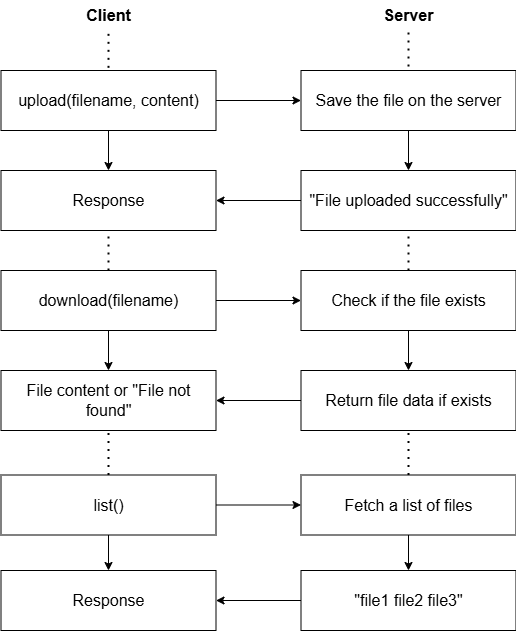
\includegraphics[width=\textwidth]{rpc_design.png}
    \caption{RPC Service Design}
    \label{fig:rpc}
\end{figure}

\section*{System Organization}
The system consists of two components:
\begin{itemize}
    \item \textbf{Server:} Hosts the XML-RPC server and implements file operations.
    \item \textbf{Client:} Connects to the server and invokes remote methods for file operations.
\end{itemize}

\begin{figure}[h]
    \centering
    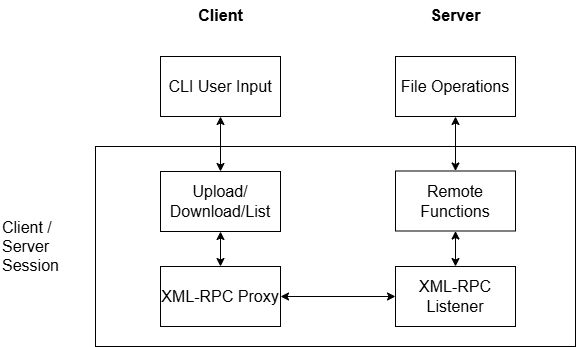
\includegraphics[width=\textwidth]{system_organization.png} % 
    \caption{System Organization}
    \label{fig:system}
\end{figure}

\section*{Implementation}
\subsection*{File Transfer Logic}
The file transfer uses Python's \texttt{xmlrpc} library, which provides built-in support for RPC communication. The server defines and registers functions for file operations, while the client connects to the server and invokes these functions.

\subsection*{Code Snippets}
\subsubsection*{Client Implementation}
\begin{lstlisting}[language=Python, caption=Client Implementation, label=lst:client, basicstyle=\ttfamily\footnotesize, keywordstyle=\color{blue}]
import xmlrpc.client
import os
from typing import Dict, Callable

ip = os.getenv("IP", "localhost")
port = int(os.getenv("PORT", 8080))


def upload(server):
    filename = input("Enter filename to upload: ").strip()

    if not os.path.exists(filename):
        return "File does not exist"

    with open(filename, "rb") as file:
        content = file.read()

    response = server.upload(filename, content)

    return response


def download(server):
    filename = input("Enter filename to download: ").strip()
    content = server.download(filename)

    if content == "File not found":
        return content
    else:
        with open(filename, "wb") as f:
            f.write(content.data)
        return f"File {filename} downloaded successfully."


def list(server):
    files = server.list()
    return files
\end{lstlisting}

\subsubsection*{Server Implementation}
\begin{lstlisting}[language=Python, caption=Server Implementation, label=lst:server, basicstyle=\ttfamily\footnotesize, keywordstyle=\color{blue}]
import xmlrpc.server
import os

def upload(filename, content):
    with open(filename, "wb") as f:
        f.write(content.data)
    return "File uploaded successfully"

def download(filename):
    if os.path.exists(filename):
        with open(filename, "rb") as f:
            content = f.read()
        return content
    else:
        return "File not found"

def list():
    files = os.listdir(".")
    return " ".join(files)

def start_server(port):
    server = xmlrpc.server.SimpleXMLRPCServer(("0.0.0.0", port), allow_none=True)
    print(f"Server started and listening on port {port}")
    server.register_function(upload, "upload")
    server.register_function(download, "download")
    server.register_function(list, "list")
    server.serve_forever()
\end{lstlisting}

\section*{Summary}
This system demonstrates a file transfer protocol using XML-RPC in Python. The implementation supports essential file operations and provides a simple and extensible architecture for future enhancements.

\end{document}
